\documentclass{article}
\usepackage[preprint]{neurips_2024}
\usepackage[utf8]{inputenc}
\usepackage[T1]{fontenc}
\usepackage{hyperref}
\usepackage{url}
\usepackage{booktabs}
\usepackage{amsfonts}
\usepackage{amsmath}
\usepackage{nicefrac}
\usepackage{microtype}
\usepackage{graphicx}
\usepackage{xcolor}
\usepackage{enumitem}

\title{PlanarBench: Evaluating LLM Spatial Reasoning\\ via Planar Graph Drawing}

\author{%
  Oleksandr Nikitin \\
  \texttt{oleksandr@tvori.info}
}

\begin{document}

\maketitle

\begin{abstract}
PlanarBench tests whether LLMs can draw planar graphs as ASCII art given only an edge list---a spatial reasoning task that resists memorization because edge order, edge orientation, and node labels are all permutable. We evaluate 91 models on the 199 simplest non-isomorphic connected planar graphs (2--7 vertices). Edge count is the dominant difficulty predictor ($r = -0.85$)---a finding not reported in prior LLM graph benchmarks, which use only node count as the difficulty axis.
\end{abstract}

%------------------------------------------------------------------
\section{Introduction}
%------------------------------------------------------------------

Spatial reasoning---the ability to mentally manipulate objects in two- or three-dimensional space---is a core component of human intelligence that remains poorly tested in LLM benchmarks. Most evaluations of LLMs on graph tasks focus on algorithmic questions: shortest paths, connectivity, cycle detection, and node classification. These tasks reduce to symbolic computation and can often be solved by memorizing algorithmic templates.

We propose a fundamentally different evaluation: given a planar graph as an edge list, produce a valid planar straight-line drawing as ASCII art. This task has several desirable properties:

\paragraph{It requires spatial reasoning.}
The model must jointly decide on node positions and mentally verify that all edges can be drawn without crossings. Algorithmic solutions exist---F\'ary's theorem~\citep{fary1948} guarantees every planar graph admits a straight-line embedding, Tutte~\citep{tutte1963} gives a constructive method for 3-connected cases, and de~Fraysseix et al.~\citep{defraysseix1990} provide a general $O(n \log n)$ algorithm producing drawings on an $O(n) \times O(n)$ grid---but the model must implicitly navigate this space without executing a known algorithm.

\paragraph{It is verifiable.}
Unlike open-ended generation tasks, correctness can be checked mechanically: parse the ASCII art, extract node coordinates and edge paths, and verify they match the input graph with no missing edges, no extra edges, and no crossings.

\paragraph{It scales naturally.}
Graph drawing difficulty increases with both vertex count and edge density, providing a built-in difficulty gradient without requiring manual task design.

\paragraph{It probes multi-constraint reasoning.}
Each edge is a constraint that interacts with every other---satisfying one adjacency may block a crossing-free route for another. The model must find a globally consistent assignment, mirroring tasks like checking a specification for contradictory requirements. Our results confirm this: difficulty scales with the number of pairwise interactions (edges, $r = -0.85$), not the number of entities (vertices, $r = -0.47$). Graph drawing may thus serve as a domain-neutral probe for constraint-satisfaction capacity---one that sidesteps training-data contamination because the constraints are geometric and vertex labels are permutable.

\paragraph{It is truly out-of-distribution.}
Vertex labels can be freely permuted: \texttt{A-B, B-C, C-A} is isomorphic to \texttt{X-Y, Y-Z, Z-X}, but reusing a memorized drawing requires recognizing the isomorphism first. For general graphs this takes quasipolynomial time~\citep{babai2016}; for planar graphs it is linear~\citep{hopcroft1974}, but still requires implicitly computing a canonical form and inverting the permutation---no shortcut over direct construction. Combined with $n!$ possible labelings per graph, memorization is an unlikely strategy.

\subsection{Related Work}

Prior work evaluating LLMs on graph tasks has focused on graph computation rather than graph drawing. \citet{wang2023} introduce NLGraph, testing LLMs on graph problems (connectivity, shortest path, bipartiteness) stated in natural language. GraphArena~\citep{tang2025} tests algorithmic tasks like shortest paths, maximum flow, and NP-complete graph problems. GraphOmni~\citep{xu2026} evaluates graph-theoretic reasoning across graph types, serialization formats, and prompt schemes. All of these test symbolic/algorithmic reasoning over graphs; none involves spatial layout.

In graph visualization, \citet{fan2025} evaluate LLM-generated layouts for graph understanding, layout generation, and layout evaluation, but do not test strict planarity. \citet{dibartolomeo2023} test whether LLMs can execute steps of graph layout algorithms such as Sugiyama-style hierarchical layout, but the task is procedural rather than requiring holistic spatial reasoning.

%------------------------------------------------------------------
\section{Benchmark Design}
%------------------------------------------------------------------

\subsection{Task Formulation}

Each benchmark instance consists of:
\begin{itemize}[nosep]
  \item \textbf{Input:} A planar graph specified as an edge list (e.g., \texttt{A - B, A - C, B - C, C - D}).
  \item \textbf{Prompt:} \texttt{"this is a graph: [edge list]. draw an ascii art representation of it, enclosed in a code block. avoid intersections, this is a planar graph."}
  \item \textbf{Expected output:} A code block containing ASCII art where each node appears exactly once as a single letter at a distinct position; edges are drawn using \texttt{-} (horizontal), \texttt{|} (vertical), \texttt{/} (diagonal up), or \texttt{\textbackslash} (diagonal down); all edges from the input graph are present; and no spurious edges are detected.
\end{itemize}

\subsection{Graph Corpus}

Our graphs are a prefix of the complete catalog of all non-isomorphic connected planar graphs, generated by \texttt{plantri}~\citep{brinkmann2007,mckay2024} and stored in graph6 format~\citep{mckay2014}. The evaluated set includes all such graphs on 2--6 vertices and the first 71 of 646 on 7 vertices, for 199 graphs total (Table~\ref{tab:vertex-dist}).

\begin{table}[h]
\centering
\caption{Distribution of benchmark graphs by vertex count.}
\label{tab:vertex-dist}
\small
\begin{tabular}{@{}lrr@{}}
\toprule
Vertices & Count & Cumulative \\
\midrule
2 & 1 & 1 \\
3 & 2 & 3 \\
4 & 6 & 9 \\
5 & 20 & 29 \\
6 & 99 & 128 \\
7 & 71 & 199 \\
\bottomrule
\end{tabular}
\end{table}

We did not extend beyond 7 vertices because the current set already saturates model capability: even with relaxed scoring, solve rates for 11- and 12-edge tasks remain below 2\%, and 8-vertex graphs have up to 18 edges---well past this effective ceiling. Adding larger graphs would increase the corpus without adding discriminative power at current capability levels.

\subsection{Validation Pipeline}

The validator operates in three stages:

\begin{enumerate}[nosep]
\item \textbf{Node extraction.} All \verb|\b\w+\b| tokens in the code block are extracted as node names. The validator checks for missing nodes, extra nodes, and duplicates.

\item \textbf{Edge detection.} The code block is parsed into a character grid. Node positions are identified, then edges are detected in priority order: \emph{horizontal} (same-row nodes connected by contiguous dash characters), \emph{vertical} (same-column nodes connected by pipe characters), and \emph{diagonal} (nodes in a \texttt{\textbackslash} or \texttt{/} relationship). Detected edge characters are ``consumed'' (replaced with a numeric marker) to prevent double-counting.

\item \textbf{Edge matching.} Detected edges are compared against the expected edge set. A drawing passes \emph{strict} validation only if both sets match exactly---no missing edges, no extra edges, and no unconsumed edge characters remain.
\end{enumerate}

Because strict straight-line validation penalizes drawings that are topologically correct but use L- or C-shaped edge paths (common when ASCII grid constraints make straight lines impossible), we additionally run two relaxed checks:
\begin{itemize}[nosep]
\item \textbf{Coordinate validation} checks that all desired edges can be drawn as straight lines without intersections given the node positions, and rejects extra nodes and detectable spurious edges.
\item \textbf{BFS validation} checks edge connectivity by running breadth-first search between adjacent nodes, accepting any contiguous path of edge characters (not just straight lines).
\end{itemize}
The per-task score is $\min\!\bigl(1,\;\max(\text{strict},\;\tfrac{1}{2}\text{coords} + \tfrac{1}{2}\text{bfs})\bigr)$: full credit for a correct straight-line drawing, half credit each for correct node placement and correct (possibly non-straight) edge connectivity, and zero otherwise.

%------------------------------------------------------------------
\section{Experimental Setup}
%------------------------------------------------------------------

\subsection{Models}

We evaluate 91 models released from December 2023 to December 2025, spanning major providers and architectures: Anthropic (Claude Opus~3, 4.5; Sonnet~3.5, 3.7, 4.5; Haiku~3.5, 4.5, with and without extended thinking), OpenAI (GPT-5.2~Pro, GPT-5.2, GPT-5, GPT-5~Mini, GPT-5~Nano, GPT-5~Codex, GPT-4.5~Preview, GPT-4.1/Mini/Nano, GPT-4o/Mini, o1/Mini, o3/Mini, o4~Mini), Google (Gemini~3~Pro/Flash~Preview, Gemini~2.5~Pro, Gemini~2.0~Pro, Gemini~2.0~Flash), xAI (Grok-2, Grok-3/Mini, Grok-4.1~Fast), Moonshot (K2, K2~Thinking), Aion~1.0, Quasar~Alpha, Hunyuan-T1, LFM-40B, Mercury~Coder, and open-weight models (DeepSeek~R1, R1~distills at 14B/32B/70B, DeepSeek~V3, DeepSeek~Prover~V2, DeepCoder~14B, Qwen~3~235B/32B/14B/8B/4B/1.7B, Qwen~3~Coder~480B, Qwen~3~Next~80B, Qwen~2.5~72B/Coder~7B/14B/32B, QwQ-32B, Qwerky-72B, Llama~3.1~405B, 3.1~Tulu-3~405B, 3.2~90B~Vision, 3.3~70B, 4~Maverick, 4~Scout, Gemma~3, Phi-4, Mixtral~8$\times$7B, Mistral~Small~3.1~24B, Cogito~v2.1~671B, GLM-4.5~Air, GLM-4.7, MiniMax-01, Jamba~1.6~Large, OLMo-2, Prime~Intellect~3, GPT-OSS~20B/120B).

Models are accessed via their respective APIs. Each model is run once per graph. Where models support extended thinking or ``high'' reasoning effort, both settings are tested as separate entries.

\subsection{Execution}

Each run calls the model API with the prompt, extracts the last code block from the response, validates it, and records the result (pass/fail, duration, error details) to a SQLite database. Runs already recorded for a given (model, graph\_index) pair are skipped, enabling incremental evaluation.

%------------------------------------------------------------------
\newpage
\section{Results}
%------------------------------------------------------------------

\subsection{Leaderboard}

Table~\ref{tab:leaderboard} shows the top-performing models.

\begin{table}[h]
\centering
\caption{Top 21 models by score (of 199). Full results cover 91 models.}
\label{tab:leaderboard}
\small
\begin{tabular}{@{}rlr@{}}
\toprule
Score & Model & Time (s) \\
\midrule
159.5 & gpt-5.2-pro-medium & 80{,}028 \\
151.0 & gemini3-pro-preview & 8{,}956 \\
144.0 & opus-4-5-32k-stream & 29{,}292 \\
130.0 & gpt-5-codex & 106{,}930 \\
127.0 & gpt-5-codex-high & 98{,}787 \\
124.5 & gpt-5-2025-08-07 & 37{,}875 \\
124.0 & gpt-5-2025-08-07-high & 50{,}602 \\
112.5 & sonnet-4-5-32k-stream & 21{,}423 \\
111.0 & gpt-5-mini-2025-08-07-high & 50{,}982 \\
101.5 & gpt-5.2-low & 9{,}616 \\
96.0 & gemini-2.5-pro-preview-05-06 & 15{,}813 \\
95.5 & sonnet-3-7-0219-32k & 24{,}942 \\
93.5 & o4-mini & 11{,}622 \\
91.0 & o1 & 19{,}255 \\
85.0 & gemini-2.5-pro-preview-03-25 & 6{,}380 \\
84.0 & glm-4.7 & 224{,}486 \\
83.5 & haiku-4-5-32k-stream & 15{,}374 \\
82.0 & gpt-5-nano-2025-08-07-high & 28{,}716 \\
81.0 & o3 & 33{,}736 \\
80.0 & grok-4-1-fast & 34{,}905 \\
78.0 & k2-thinking & 45{,}220 \\
\bottomrule
\end{tabular}
\end{table}

\subsection{Key Findings}

\paragraph{Finding 1: Extended thinking and model scale both improve spatial reasoning.}
Sonnet~3.7 jumps from 39.5/199 without thinking to 95.5/199 with 32k thinking tokens---by far the largest gain from reasoning effort alone. Moonshot K2 shows a similar leap (25.0 $\to$ 78.0 with thinking), and GPT-5~Mini improves substantially (78.0 $\to$ 111.0 with ``high'' reasoning). Within a model family at fixed thinking budget, scale matters: Opus~4.5 (144.0) $>$ Sonnet~4.5 (112.5) $>$ Haiku~4.5 (83.5), all with 32k tokens. However, thinking does not help uniformly: GPT-5~``high'' (124.0) matches base GPT-5 (124.5), suggesting the benefit depends on model architecture.

\paragraph{Finding 2: Spatial reasoning does not track standard benchmark rankings.}
Claude Opus~4.5 (144.0/199) outperforms GPT-5 (124.5/199) on PlanarBench despite scoring lower on the Artificial Analysis Intelligence Index (43 vs.\ 45). The o1 model (91.0/199) underperforms Sonnet~3.7 with extended thinking (95.5/199). Standard leaderboard positions are poor predictors of spatial layout ability.

\paragraph{Finding 3: A capability cliff exists around 30B parameters.}
Models below 30B parameters almost universally score under 20/199: Phi-4 (13.5), Gemma~3 (12.0), Qwen~2.5~Coder~32B (17.0). The smallest models (7B range) score under 11. Spatial reasoning appears to require a minimum representational capacity that small models lack.

\paragraph{Finding 4: Edge count is the primary difficulty driver.}
The Pearson correlation between a task's edge count and its score (averaged across all models) is $r = -0.85$, 95\% CI $[-0.88, -0.80]$. By comparison, vertex count alone correlates at only $r = -0.47$ $[-0.57, -0.36]$---the confidence intervals do not overlap. After controlling for vertex count via partial correlation, edge count retains $r = -0.80$ $[-0.84, -0.74]$.

Table~\ref{tab:binned} shows the binned solve rates, and Figures~\ref{fig:bar} and~\ref{fig:scatter} visualize the relationship. Bins with $n = 1$ have no meaningful CI. The 3-edge bin ($n = 3$) has a wide interval; bins with $n \ge 5$ have CIs within $\pm$6 percentage points.

Even under relaxed scoring, the transition from ``usually solvable'' ($\le$5 edges) to ``rarely solved'' ($\ge$9 edges) spans a narrow range. Tasks with 11--12 edges see solve rates below 2\%, suggesting a near-hard threshold in current model capability.

\begin{table}[h]
\centering
\caption{Mean score by edge count (across all models). Bins with $n=1$ have no meaningful CI.}
\label{tab:binned}
\small
\begin{tabular}{@{}rrrr@{}}
\toprule
Edges & Tasks & Mean Score & 95\% CI \\
\midrule
1 & 1 & 92.0\% & --- \\
2 & 1 & 84.2\% & --- \\
3 & 3 & 73.9\% & [56.2\%, 91.6\%] \\
4 & 5 & 55.0\% & [43.6\%, 66.4\%] \\
5 & 12 & 46.4\% & [42.2\%, 50.7\%] \\
6 & 26 & 36.4\% & [31.5\%, 41.4\%] \\
7 & 39 & 27.1\% & [23.5\%, 30.7\%] \\
8 & 43 & 16.3\% & [13.3\%, 19.3\%] \\
9 & 35 & 8.3\% & [5.9\%, 10.7\%] \\
10 & 21 & 5.1\% & [2.3\%, 7.9\%] \\
11 & 10 & 1.6\% & [0.6\%, 2.5\%] \\
12 & 3 & 1.0\% & [1.0\%, 1.0\%] \\
\bottomrule
\end{tabular}
\end{table}

\begin{figure}[t]
\centering
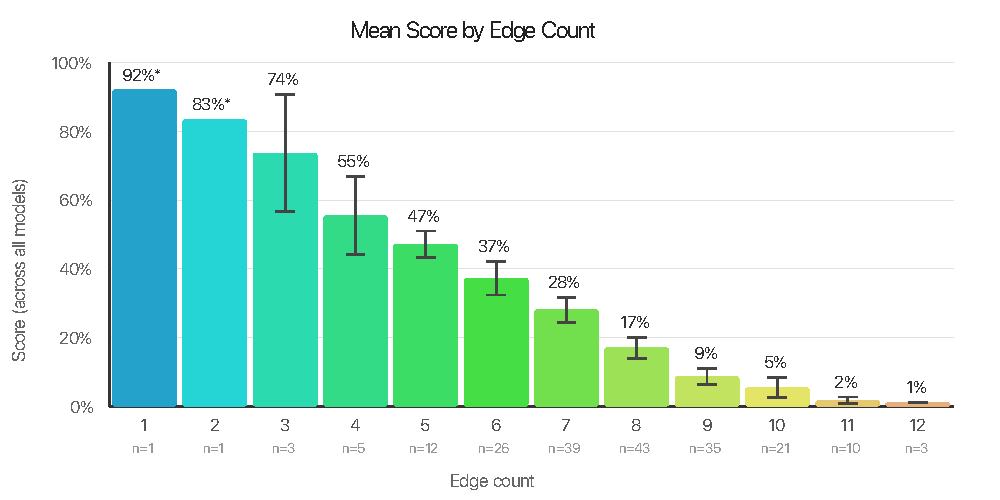
\includegraphics[width=\linewidth]{fig-solve-rate-by-edges-bar.pdf}
\caption{Mean score (across all models) decreases monotonically with edge count. Error bars show 95\% CIs; asterisked bars ($n=1$) have no CI. Sample sizes shown below each bar.}
\label{fig:bar}
\end{figure}

\begin{figure}[t]
\centering
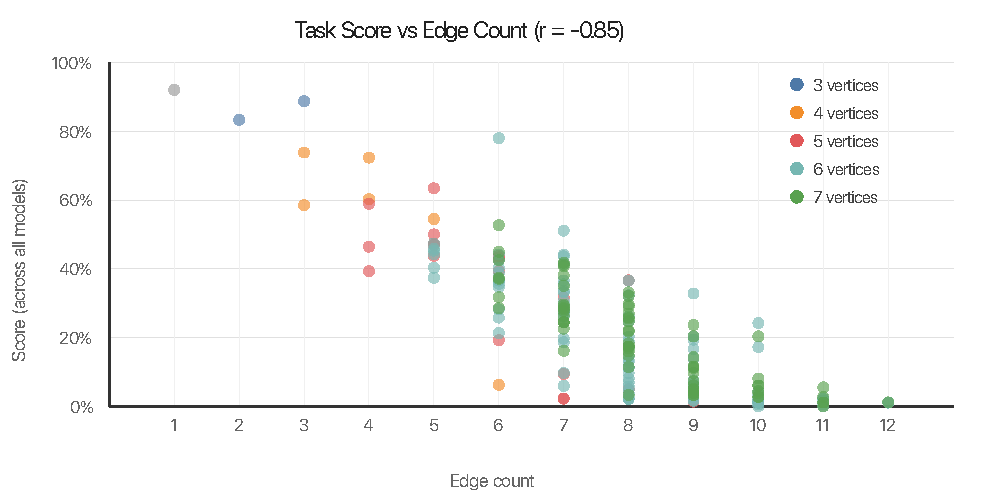
\includegraphics[width=\linewidth]{fig-solve-rate-vs-edges-scatter.pdf}
\caption{Each point is one benchmark task, colored by vertex count. The strong negative correlation ($r = -0.85$) holds within every vertex group, confirming that edge density---not just graph size---drives difficulty.}
\label{fig:scatter}
\end{figure}

\paragraph{Finding 5: Cost-efficiency varies enormously.}
Gemini~3~Pro~Preview achieves the second-highest score (151.0/199) in 8{,}956 seconds of total API time. GPT-5~Codex achieves a comparable score (130.0/199) but takes 106{,}930 seconds---over 11$\times$ slower. Prime Intellect~3 achieves 74.0/199 in 150{,}475 seconds. Speed and quality are not correlated (Figure~\ref{fig:time}).

\begin{figure}[t]
\centering
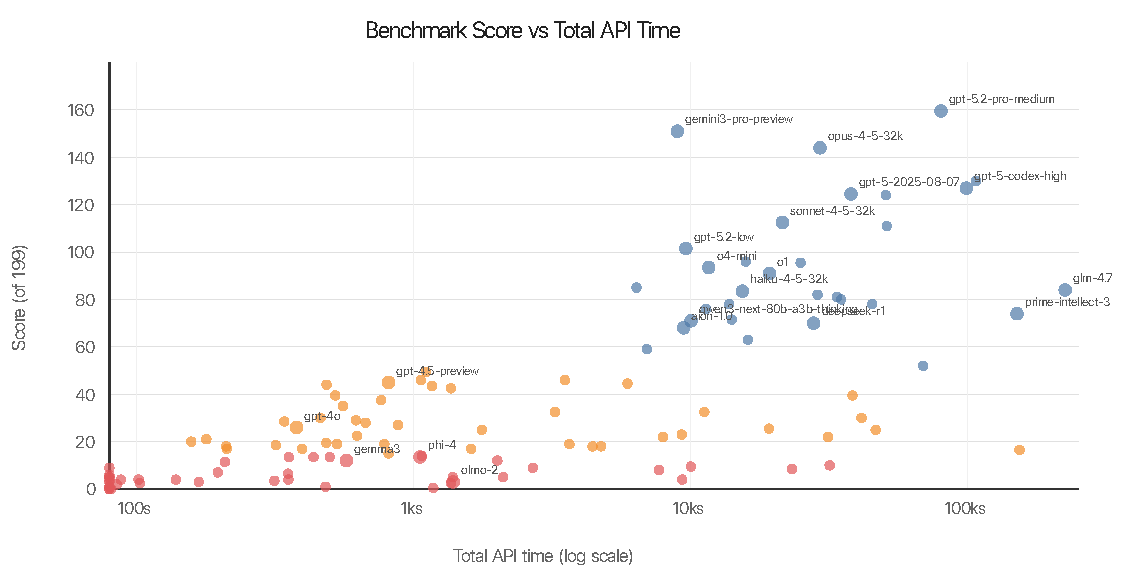
\includegraphics[width=\linewidth]{fig-solved-vs-time-scatter.pdf}
\caption{Each point is one model. The $x$-axis (log scale) shows total API wall-clock time; the $y$-axis shows score. Colors indicate score tiers: blue (50+), orange (15--49), red ($<$15).}
\label{fig:time}
\end{figure}

\begin{figure}[t]
\centering
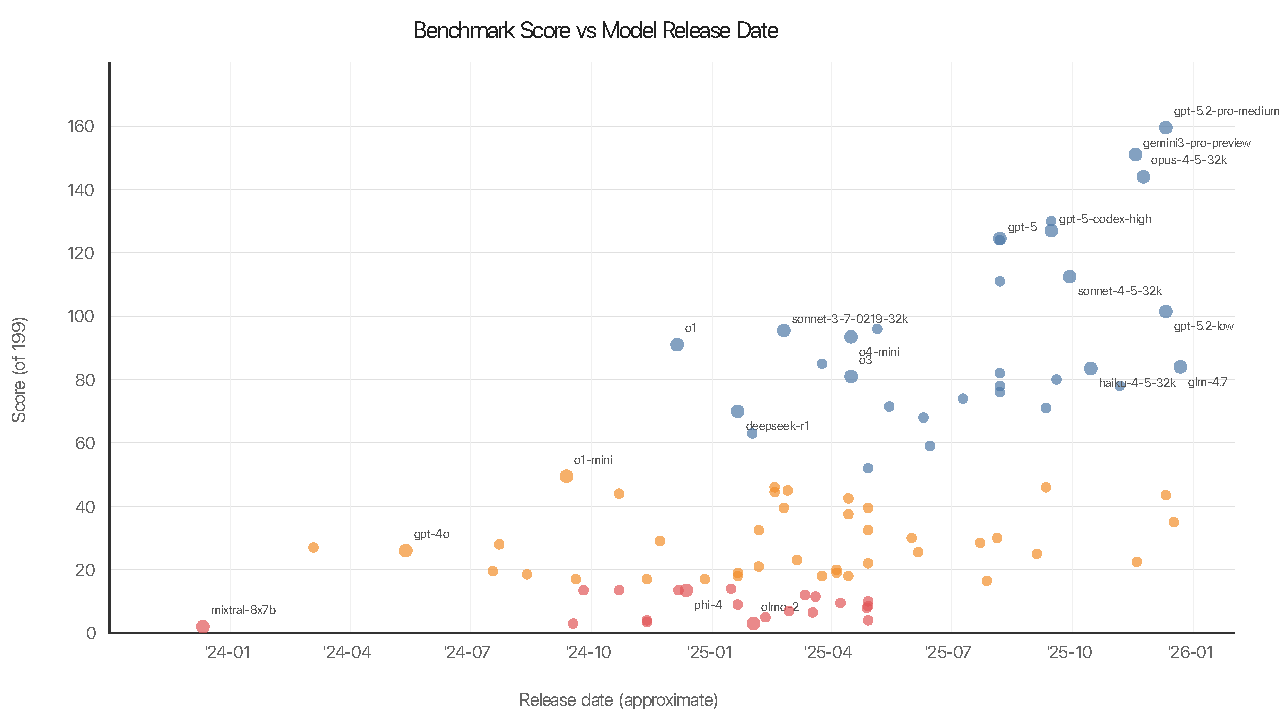
\includegraphics[width=\linewidth]{fig-solved-vs-release-date-scatter.pdf}
\caption{Score vs model release date. Newer models score higher, and with the exception of o1 the frontier is almost linearly growing.}
\label{fig:release}
\end{figure}

\subsection{Error Analysis}

Common failure modes include:
\begin{itemize}[nosep]
\item \textbf{Missing edges:} The model places nodes correctly but fails to connect all required pairs---the most common failure, particularly for high-degree nodes.
\item \textbf{Extra edges:} The model draws connections not in the input graph, often because dash characters in ``decorative'' spacing are parsed as edges.
\item \textbf{Node placement failures:} Missing or duplicate node labels, particularly when models add annotations outside the intended drawing area.
\item \textbf{Broken edges:} Edge characters that don't form a contiguous path between their endpoints---a dash or pipe that is slightly misaligned.
\end{itemize}

%------------------------------------------------------------------
\newpage
\section{Discussion}
%------------------------------------------------------------------

\subsection{Why ASCII Art?}

We chose ASCII art over coordinate-pair output for several reasons. First, ASCII art is a practical output modality---it is widely used for diagrams and documentation, and LLMs encounter it in training data. Second, it tightly couples node placement with edge routing: the model must simultaneously reason about where nodes go and whether edges can be drawn between them without crossing.

The downside is that ASCII art constrains the space of valid drawings. Diagonal edges must use \texttt{/} and \texttt{\textbackslash} characters, which limits angular resolution. Some planar embeddings (e.g.\ the complete $K_4$ graph) that would be easy to draw on a continuous 2D canvas are hard to express in ASCII. To account for this, our scoring awards partial credit for drawings with correct node placement or correct edge connectivity via non-straight paths (see Section~2.3). This arguably makes the benchmark \emph{harder} than coordinate-based alternatives, which we view as acceptable---a benchmark where the best model scores 159.5 of 199 is more informative than one they solve nearly all of. The open-ended design of the benchmark was inspired by AidanBench~\citep{mclaughlin2025aidanbench}, and the idea originally arose in the context of LLM-assisted requirements engineering, where we observed a correlation between a model's ability to render dependency diagrams correctly and its ability to spot contradictions between task statements.

\subsection{Edge Density as the True Difficulty Axis}

Vertex count alone is a weak predictor of difficulty (Pearson $r = -0.47$), while edge count dominates ($r = -0.85$). The partial correlation of edge count with score, controlling for vertices, remains strong at $r = -0.80$ $[-0.84, -0.74]$.

Each additional edge constrains the layout more tightly, reducing the space of valid planar embeddings. A 7-vertex tree (6~edges) is far easier to draw than a 6-vertex maximal planar graph (12~edges), despite having more nodes. The combinatorial bottleneck is not ``where to put the nodes'' but ``how to route all edges without crossings given the node positions.''

Even with relaxed scoring that recognizes non-straight edge connectivity and edges skipped due to acute angles, tasks with 11--12 edges see scores below 2\%, suggesting that current models hit a near-hard limit in their spatial reasoning capacity at this edge density.

\subsection{Limitations}

\begin{itemize}[nosep]
\item \textbf{Single-attempt evaluation.} Each model gets one attempt per graph. Some models might succeed on retry with different sampling. Broader multi-attempt evaluation was constrained by the API costs of frontier reasoning models. Future work could evaluate pass@$k$.
\item \textbf{ASCII-specific failures.} Some failures reflect difficulty with the ASCII medium rather than spatial reasoning per se. The relaxed scoring (coordinate and BFS checks) partially addresses this by awarding credit when topology is correct but edge paths are non-straight.
\item \textbf{Graph size.} The current benchmark maxes out at 7 vertices. However, the benchmark is open-ended by design: McKay's corpus contains 71{,}885 planar graphs at 9 vertices and the counts grow super-exponentially, so the task set can be extended indefinitely as models improve. Scaling beyond ASCII would require switching to a coordinate-output format.
\item \textbf{Prompt sensitivity.} We use a single, simple prompt. Prompt engineering (e.g., chain-of-thought, few-shot examples) might improve results but was not explored.
\end{itemize}

%------------------------------------------------------------------
\section{Conclusion}
%------------------------------------------------------------------

Planar graph drawing is a discriminating test of LLM capabilities: simple to state, easy to verify, difficult to solve via memorization, and it exposes a wide performance spread across models. Edge density is the primary difficulty driver ($r = -0.85$), with scores below 2\% for tasks with 11+ edges even under relaxed scoring. Prior LLM graph benchmarks (GraphArena, NLGraph, GraphOmni) use node count as the sole difficulty axis; our results show that edge count is a stronger predictor and remains dominant after controlling for vertex count. Extended thinking and model scale are the dominant predictors of success, and the ranking on this spatial task diverges meaningfully from standard LLM leaderboards.

PlanarBench is open-ended: since the number of planar graphs grows super-exponentially with vertex count, the benchmark can be extended indefinitely to challenge more powerful future models without redesigning the task or evaluation. We release the graph corpus and evaluation harness at \url{https://github.com/wizzard0/planar-bench-as1073} to support further research on spatial reasoning in language models.

%------------------------------------------------------------------
\newpage
\bibliographystyle{plainnat}

\begin{thebibliography}{14}

\bibitem[Babai(2016)]{babai2016}
L.~Babai.
\newblock Graph isomorphism in quasipolynomial time.
\newblock In \emph{Proceedings of the 48th Annual ACM Symposium on Theory of Computing (STOC)}, pp.\ 684--697, 2016.

\bibitem[Brinkmann \& McKay(2007)]{brinkmann2007}
G.~Brinkmann and B.~D. McKay.
\newblock Fast generation of planar graphs.
\newblock \emph{MATCH Communications in Mathematical and in Computer Chemistry}, 58(2):323--357, 2007.

\bibitem[de~Fraysseix et~al.(1990)]{defraysseix1990}
H.~de~Fraysseix, J.~Pach, and R.~Pollack.
\newblock How to draw a planar graph on a grid.
\newblock \emph{Combinatorica}, 10(1):41--51, 1990.

\bibitem[Di~Bartolomeo et~al.(2023)]{dibartolomeo2023}
S.~Di~Bartolomeo, G.~Severi, V.~Schetinger, and C.~Dunne.
\newblock Ask and you shall receive (a graph drawing): Testing {ChatGPT}'s potential to apply graph layout algorithms.
\newblock In \emph{EuroVis 2023 Short Papers}, 2023.

\bibitem[Fan et~al.(2025)]{fan2025}
Y.~Fan, X.~Lyu, L.~Wang, Y.~Zhao, F.~Zhou, and Y.~Wang.
\newblock How well will {LLM}s perform for graph layout tasks?
\newblock \emph{Visual Informatics}, 100285, 2025.

\bibitem[F\'ary(1948)]{fary1948}
I.~F\'ary.
\newblock On straight-line representation of planar graphs.
\newblock \emph{Acta Scientiarum Mathematicarum (Szeged)}, 11(4):229--233, 1948.

\bibitem[Hopcroft \& Wong(1974)]{hopcroft1974}
J.~E. Hopcroft and J.~K. Wong.
\newblock Linear time algorithm for isomorphism of planar graphs (preliminary report).
\newblock In \emph{Proceedings of the 6th Annual ACM Symposium on Theory of Computing (STOC)}, pp.\ 172--184, 1974.

\bibitem[McKay(2024)]{mckay2024}
B.~D. McKay.
\newblock Combinatorial data: Planar graphs.
\newblock Australian National University, 2024.
\newblock \url{https://users.cecs.anu.edu.au/~bdm/data/graphs.html}.

\bibitem[McKay \& Piperno(2014)]{mckay2014}
B.~D. McKay and A.~Piperno.
\newblock Practical graph isomorphism, {II}.
\newblock \emph{Journal of Symbolic Computation}, 60:94--112, 2014.

\bibitem[McLaughlin et~al.(2024)]{mclaughlin2025aidanbench}
A.~McLaughlin, J.~Campbell, A.~Uppuluri, and Y.~Yang.
\newblock {AidanBench}: Stress-testing language model creativity on open-ended questions.
\newblock In \emph{NeurIPS 2024 Workshop on Language Gamification}, 2024.
\newblock \url{https://github.com/aidanmclaughlin/AidanBench}.

\bibitem[Tang et~al.(2025)]{tang2025}
J.~Tang, Q.~Zhang, Y.~Li, N.~Chen, and J.~Li.
\newblock {GraphArena}: Evaluating and exploring large language models on graph computation.
\newblock In \emph{International Conference on Learning Representations (ICLR)}, 2025.

\bibitem[Tutte(1963)]{tutte1963}
W.~T. Tutte.
\newblock How to draw a graph.
\newblock \emph{Proceedings of the London Mathematical Society}, s3-13(1):743--767, 1963.

\bibitem[Wang et~al.(2023)]{wang2023}
H.~Wang, S.~Feng, T.~He, Z.~Tan, X.~Han, and Y.~Tsvetkov.
\newblock Can language models solve graph problems in natural language?
\newblock In \emph{Advances in Neural Information Processing Systems (NeurIPS)}, 2023.

\bibitem[Xu et~al.(2026)]{xu2026}
H.~Xu, X.~Jian, X.~Zhao, W.~Pang, C.~Zhang, S.~Wang, Q.~Zhang, Z.~Dong, J.~Monteiro, B.~Liu, Q.~Sun, and T.~Yu.
\newblock {GraphOmni}: A comprehensive and extensible benchmark framework for large language models on graph-theoretic tasks.
\newblock In \emph{International Conference on Learning Representations (ICLR)}, 2026.

\end{thebibliography}

%------------------------------------------------------------------
\newpage
\appendix
\section{Relaxed Validation Examples}
\label{app:examples}
%------------------------------------------------------------------

The following examples illustrate drawings that fail strict validation but pass one or both relaxed checks. Each category is named by its (strict, coordinate, BFS) pass/fail pattern.

\subsection*{Category 0-0-1: BFS only}

These drawings fail both strict and coordinate checks but pass BFS validation, typically because an edge is routed around an intervening node rather than drawn as a straight line.

\paragraph{Task 17 (5 nodes).} Coordinate check rejects edge D--E because the straight line passes through B; BFS recovers the outside route.

\begin{verbatim}
           D---------+
          /|\        |
         / | \       |
        A  B  C      |
         \ | /       |
          \|/        |
           E---------+
\end{verbatim}

\paragraph{Task 126 (6 nodes).} Coordinate check rejects A--B by straight-line intersection; BFS accepts the outer routed path.

\begin{verbatim}
                 A-----------+
                / \          |
               /   \         |
              /     \        |
             C--------E      |
             |      / |      |
             |     /  |      |
             |    /   |      |
             |   /    |      |
             |  /     |      |
             | /      |      |
             |/       |      |
             F--------D      |
              \      /       |
               \    /        |
                \  /         |
                 B-----------+
\end{verbatim}

\paragraph{Task 159 (7 nodes).} Coordinate check rejects E--F because the straight segment passes through C; BFS accepts the routed bottom edge.

\begin{verbatim}
    A       B
     \     /
      G   F
     /|\ /|
    D | C |
     \|   |
      E---'
\end{verbatim}
\newpage
\subsection*{Category 0-1-0: Coordinate only}

These drawings have valid node placements (all desired edges can be drawn as non-intersecting straight lines), but BFS cannot find a drawn path for every edge.

\paragraph{Task 22 (5 nodes).} Coordinates are acceptable, but BFS does not find D--E as a drawn edge.

\begin{verbatim}
       A
      / \
     C - E
    /     \
   D-------B
\end{verbatim}

\paragraph{Task 62 (6 nodes).} Coordinates are acceptable, but BFS misses C--F.

\begin{verbatim}
        A
        |
        F
       /|\ \
      / | \ \
     /  |  \ \
    /   |   \ \
   B----D----E----C
\end{verbatim}

\paragraph{Task 187 (7 nodes).} Coordinates are acceptable, but BFS misses F--G and C--E.

\begin{verbatim}
          A
          |
          |
          |
          |
    C-----G-----B
    |    /|\
    |   / | \
     \ /  |  \
      E   |   D
      |    \ /
      +-----F
\end{verbatim}
\newpage
\subsection*{Category 0-1-1: Coordinate and BFS}

These drawings pass both relaxed checks but fail strict validation, typically because edges use L-shaped or routed paths rather than straight-line ASCII characters.

\paragraph{Task 3 (3 nodes).} BFS recovers the routed B--C edge via the corner.

\begin{verbatim}
A---B
|   |
C---+
\end{verbatim}

\paragraph{Task 5 (4 nodes).} Can be drawn with straight lines, but needs BFS to recognize paths for A--D and C--D.

\begin{verbatim}
A---+
    |
    D---B
    |   |
    |   |
    +---C
\end{verbatim}

\paragraph{Task 166 (7 nodes).} Can be drawn with straight lines, but needs BFS to recognize the angled D--E and E-G edges.

\begin{verbatim}
      A
      |
D-----F-----G
|     |    /|\
|     |   / | \
+-----E--/  C  B
\end{verbatim}

\end{document}
